\documentclass{article}
\usepackage{../verslagstyle}



\begin{document}
	\title{Labo 5}
	\author{Bert De Saffel}
	\date{11 maart 2019}
	\maketitle
	
	\section*{Oefening 10}
	Ik heb een functie \texttt{getDoGFilter(size, sigmabig, sigmasmall, angle)} gemaakt die de DogFilter zal aanmaken. Deze functie voert stapsgewijs de procedure van de opdracht uit. 
	\subsection*{Nieuwe functies}
	\begin{itemize}
		 \item \textbf{getGaussianKernel(ksize, sigma) $\rightarrow$ retval}
		 
		 Genereert een kolommatrix met $ksize$ rijen. De matrix wordt gedefinieerd als
		 $$G_i = \alpha * \exp\bigg(-\frac{(i - (ksize - 1)/2)^2}{2*\sigma^2}\bigg)$$ 
		 \item \textbf{getRotationMatrix2D(center, angle, scale) $\rightarrow$ retval}
		 
		 Genereert een $2 \times 3$ matrix van een twee-dimensionale rotatie. De \textit{center} parameter stelt het rotatiepunt voor, de \textit{angle} parameter de rotatiehoek en de \textit{scale} parameter de schaal. De gegenereerde matrix heeft volgende vorm:
		 $$\begin{bmatrix}
		 \alpha & \beta & (1 - \alpha)\cdot center\cdot x - \beta \cdot center\cdot y \\
		 -\beta & \alpha & \beta\cdot center\cdot x - (1 - \alpha) \cdot center\cdot y
		 \end{bmatrix}$$
		 met
		 $$\alpha = scale\cdot\cos(angle)$$
		 $$\beta = scale\cdot\sin(angle)$$
	\end{itemize}
	
	\subsection*{Invoer en uitvoer}
			\begin{figure}[!htb]
		\begin{minipage}{0.48\textwidth}
			\centering
			
\includegraphics[width=0.9\linewidth]{rays}
			\caption{Originele image.}
		\end{minipage}\hfill
		\begin{minipage}{0.48\textwidth}
			\centering
			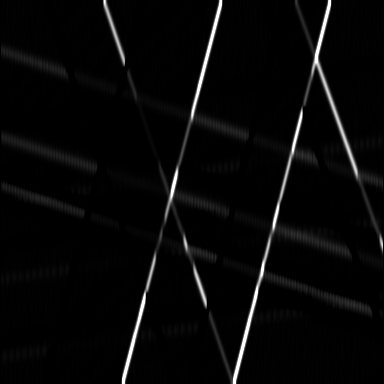
\includegraphics[width=0.9\linewidth]{raysEX10}
			\caption{De randen van de gele strepen.}
		\end{minipage}
	\end{figure}
	\newpage
	\section*{Oefening 11}
	De functie \texttt{detectLines(image, threshold1, threshold2) $\rightarrow$ dst} is een eigen wrapperfunctie die de lijnen zal detecteren. De randen worden bepaald met de Canny functie. De lijnen worden dan bepaald met de HoughLines functie. Het resultaat van HoughLines is een verzameling lijnen in de Houghruimte die elk gekarakteriseerd kunnen worden door $\rho$ en $\theta$. De vergelijking van zo een rechte is:
	$$\rho = x\cos(\theta) + y\sin(\theta)$$
	Om nu lijnen te kunnen tekenen op de figuur wordt eerst de vergelijking omgevormd in $y = ax + b$ vorm:
	$$y = -x\cot(\theta) + \frac{\rho}{\sin(\theta)}$$
	Hierbij is $a = -\cot(\theta)$ en $b = \rho/\sin(\theta)$.
	In Python kan een anonieme functie aangemaakt worden:
	$$\texttt{y = lambda x : a*x + b}$$
	Als we nu voor elke lijn in de Houghruimte twee punten zoeken waarbij $x_0 = 1$ en $x_1 = width$ en $width$ de breedte is van de image, dan kunnen de twee punten in de beeldruimte gedefinieerd worden als:
	$$\texttt{point1 = (x0, y(x0))}$$
	$$\texttt{point2 = (x1, y(x1))}$$
	Deze punten kunnen dan meegegeven worden aan de \texttt{line} functie van openCV. De lijnen zullen automatisch geclipped worden.
	\subsection*{Nieuwe functies}
	\begin{itemize}
	\item \textbf{Canny(image, threshold1, threshold2, ..., L2gradient) $\rightarrow$ edges}

	Deze functie zoekt randen in een figuur via het Canny algoritme. De hysteresis procedure vraagt om twee thresholds om pixels met een te lage waarde (threshold1) te verwerpen en die met een hoge waarde (threshold2) bij te houden.
	\item \textbf{HoughLines(image, rho, theta, threshold) $\rightarrow$ lines}
	
	Deze functie zoekt lijnen in een figuur. De parameters $\rho$ en $\theta$ specificeren de resolutie van de Houghruimte.
	
	
	\item \textbf{line(img, pt1, pt2, color) $\rightarrow$ None}
	
	Tekent een lijnsegment op de opgegeven image. Deze functie verwacht de coördinaten van twee punten en RGB kleur van de lijn.
	\end{itemize}
	\subsection*{Invoer en uitvoer}
	\begin{figure}[!htb]
		\begin{minipage}{0.48\textwidth}
			\centering
			
\includegraphics[width=0.9\linewidth]{rays}
			\caption{Originele image.}
		\end{minipage}\hfill
		\begin{minipage}{0.48\textwidth}
			\centering
			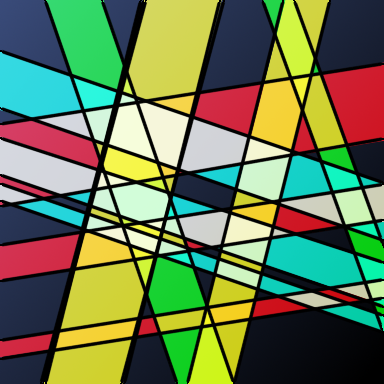
\includegraphics[width=0.9\linewidth]{raysEX11}
			\caption{Gedetecteerde lijnen.}
		\end{minipage}
	\end{figure}
	\newpage
	\section*{Oefening 12}
	De wrapperfunctie \texttt{detectCorners(image)} voert het algoritme uit om de hoekpunten te bepalen. Deze functie maakt gebruik van \texttt{goodFeaturesToTrack()} om de coördinaten van de hoekpunten te bepalen. Deze hoekpunten worden dan omcirkeld via de functie \texttt{circle()}
	\subsection*{Nieuwe functies}
	\begin{itemize}

		
		\item \textbf{goodFeaturesToTrack(image, maxCorners, qualityLevel, minDistance) $\rightarrow$ corners}
		
		Deze functie bepaalt hoeken in een beeld. De \textit{maxCorners} parameter bepaalt het aantal hoeken dat gevonden moet worden, de \textit{qualityLevel} parameter zet een threshold op de waarde van de kwaliteit van een hoek en de \textit{minDistance} parameter bepaalt minimum afstand tussen twee hoeken. 
		\item \textbf{circle(img, center, radius, color) $\rightarrow$ None}
		
		Tekent een cirkel op de opgegeven image. De \textit{center} parameter zijn de middelpuntcoördinaten van de cirkel, de \textit{radius} parameter is de straal van de cirkel en de \textit{color} parameter bevat de RGB kleur van de cirkel.	 
	\end{itemize}
	
	\subsection*{Invoer en uitvoer}
		\begin{figure}[!htb]
		\begin{minipage}{0.48\textwidth}
			\centering
			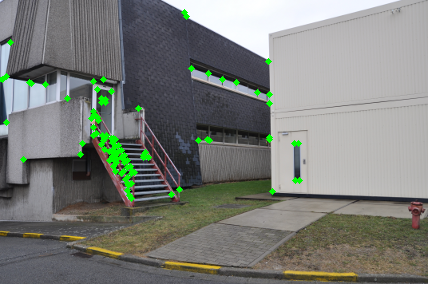
\includegraphics[width=0.9\linewidth]{shot1EX12}
			\caption{Hoekdetectie voor shots1.png.}
		\end{minipage}\hfill
		\begin{minipage}{0.48\textwidth}
			\centering
			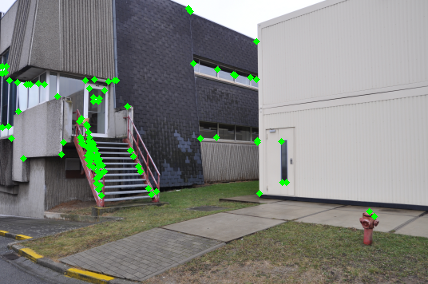
\includegraphics[width=0.9\linewidth]{shot2EX12}
			\caption{Hoekdetectie voor shots2.png.}
		\end{minipage}
	\end{figure}
	\newpage
	\section*{Oefening 13}
	\subsection*{Nieuwe functies}
	\begin{itemize}		
		\item \textbf{ORB}
		\item \textbf{BFMatcher}
		\item \textbf{drawMatches}
	\end{itemize}
	\subsection*{Invoer en uitvoer}
	\begin{figure}[!htb]
			\centering
			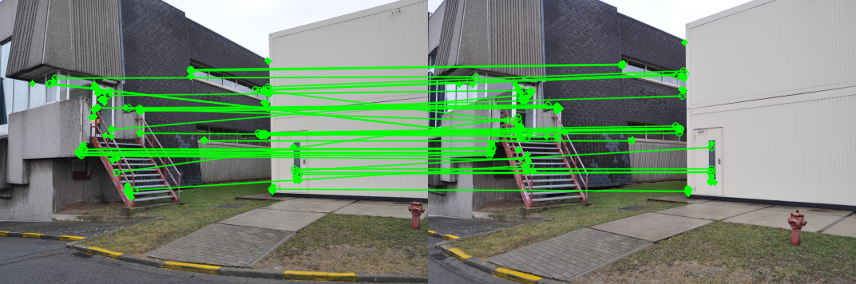
\includegraphics[width=\linewidth]{matchesEX13}
			\caption{Hoekmatches voor shots1.png en shots2.png.}
	\end{figure}

	
\end{document}